\chapter{Implementasi dan Pengujian}
\label{chap:implementasi}

Bab ini terdiri dari dua bagian, yaitu Implementasi Perangkat Lunak dan Pengujian Perangkat Lunak. Bagian implementasi berisi penjelasan lingkungan implementasi dan hasil implementasi. Sedangkan bagian pengujian berisi hasil pengujian fungsional dan eksperimental terhadap perangkat lunak yang telah dibangun.

\section{Implementasi}

\subsection{Lingkungan Implementasi}

Lingkungan implementasi terbagi menjadi dua bagian, yaitu lingkungan perangkat keras dan lingkungan perangkat lunak. Kedua bagian tersebut akan dijelaskan sebagai berikut:
\begin{enumerate}
	\item \textbf{Lingkungan Perangkat Keras} \\
	\begin{enumerate}
		\item \textbf{Komputer}: Macbook Pro (Retina, 13 inch, Mid 2014)
		\item \textbf{Prosesor}: 2.6 GHz Intel Core i5
		\item \textbf{Memori}: 8 GB 1600 MHz DDR3
		\item \textbf{Grafis}: Intel Iris 1536 MB
	\end{enumerate}

	\item \textbf{Lingkungan Perangkat Lunak} \\
	Lingkungan perangkat lunak terbagi menjadi dua bagian yaitu, lingkungan pada \textit{server} dan \textit{client}. Kedua bagian tersebut akan dijelaskan sebagai berikut:
	\begin{enumerate}
		\item \textbf{Server} \\
		\begin{enumerate}
			\item \textbf{Heroku} \\
			Heroku merupakan \textit{cloud platform} yang menyediakan fitur yang dapat membantu pengguna untuk dapat memiliki alamat domain. Spesifikasi Heroku yang digunakan oleh Finger For Life akan dijelaskan sebagai berikut:
			
			\begin{tabular}{ |p{1.5cm}|p{1.5cm}|p{2cm}|p{1.5cm}|p{1.5cm}|p{1.5cm}|p{1.5cm}|}
			\hline
			Dyno Type & Sleeps & Professional Features & Memory (RAM) & CPU Share & Dedicated & Compute \\ \hline
			free & yes & no & 512 MB & 1x & no & 1x-4x \\ \hline
				
			\end{tabular}
			
			\item \textbf{Node.js} \\
			Node.js merupakan JavaScript \textit{runtime} yang menyediakan fitur untuk mengeksekusi JavaScript dilingkungan lokal. Pengembangan Finger For Life menggunakan Node.js sebagai dasar penggunaan JavaScript dalam hal pengaturan \textit{server} maupun \textit{client}. Versi Node.js yang dipakai adalah 8.11.4.
			
			\item \textbf{Socket.io} \\
			Socket.io merupakan teknologi yang menyediakan fitur komunikasi dua arah secara \textit{real-time} antara \textit{client} dan \textit{server}. Pengembangan Finger For Life menggunakan Socket.io sebagai cara komunikasi berdasarkan \textit{event} antara \textit{client} dan \textit{server}. Dengan menggunakan Socket.io, maka proses komunikasi dalam permainan menjadi lebih efisien. Versi Socket.io yang dipakai adalah 2.0.4.
			 
		\end{enumerate}
		
		\item \textbf{Client}
		\begin{enumerate}
			\item \textbf{Express.js} \\
			Express.js adalah web \textit{framework} untuk Node.js. \textit{Framework} ini menyediakan kumpulan fitur yang dapat membantu dalam pembuatan aplikasi web. Pengembangan Finger For Life menggunakan Express.js untuk mengatur struktur direktori yang diperlukan. Dengan menggunakan Express.js, direktori dan berkas yang diperlukan untuk pengembangan dapat diatur peletakannya. Versi Express.js yang dipakai adalah 4.15.5.
			
			\item \textbf{Canvas API} \\
			Pengembangan Finger For Life menggunakan Canvas API untuk membuat elemen-elemen grafis didalam web. Canvas API digunakan untuk membuat animasi permainan pada saat pemain menggerakan karakter yang ada dilintasan lari.
			
			\item \textbf{jQuery} \\
			Pengembangan Finger For Life menggunakan Canvas API untuk mengatur akses elemen-elemen html yang ada didalam berkas-berkas tertentu. jQuery pun digunakan untuk mengirimkan data dalam bentuk form yang sudah diisi oleh pengguna. Versi jQuery yang dipakai adalah 3.3.1.
			
			\item \textbf{The Content Template element} \\
			Pengembangan Finger For Life menggunakan The Content Template element untuk menampilkan kumpulan elemen HTML kelayar dengan menggunakan elemen <template>. 
			
		\end{enumerate}
	\end{enumerate}
	
\end{enumerate}

\subsection{Hasil Implementasi}

Hasil implementasi berupa aplikasi berbasis web yang berjalan berdasarkan Node.js. Aplikasi dapat diakses pada jaringan internet dengan URL \url{http://fingerforlife.herokuapp.com}. Aplikasi Finger For Life terdiri dari beberapa halaman. Halaman tersebut terbagi menjadi dua bagian, yaitu halaman pada \textit{PC} dan pada \textit{smartphone}. Halaman-halaman tersebut antara lain:

\begin{enumerate}
	\item \textbf{Halaman \textit{home}} \\
	\textbf{PC} \\
	Halaman \textit{home} pada \textit{PC} digunakan pengguna untuk memulai permainan. Pada halaman ini terdapat tombol \textit{start} yang berfungsi untuk meminta akses masuk kedalam permainan. Apabila pengguna menekan tombol tersebut, maka pengguna akan diarahkan kehalaman selanjutnya. Tangkapan layar dari halaman \textit{home} pada \textit{PC} dapat dilihat pada gambar \ref{fig:realWeb1_home}.
	
\begin{figure}[H]
	\centering
	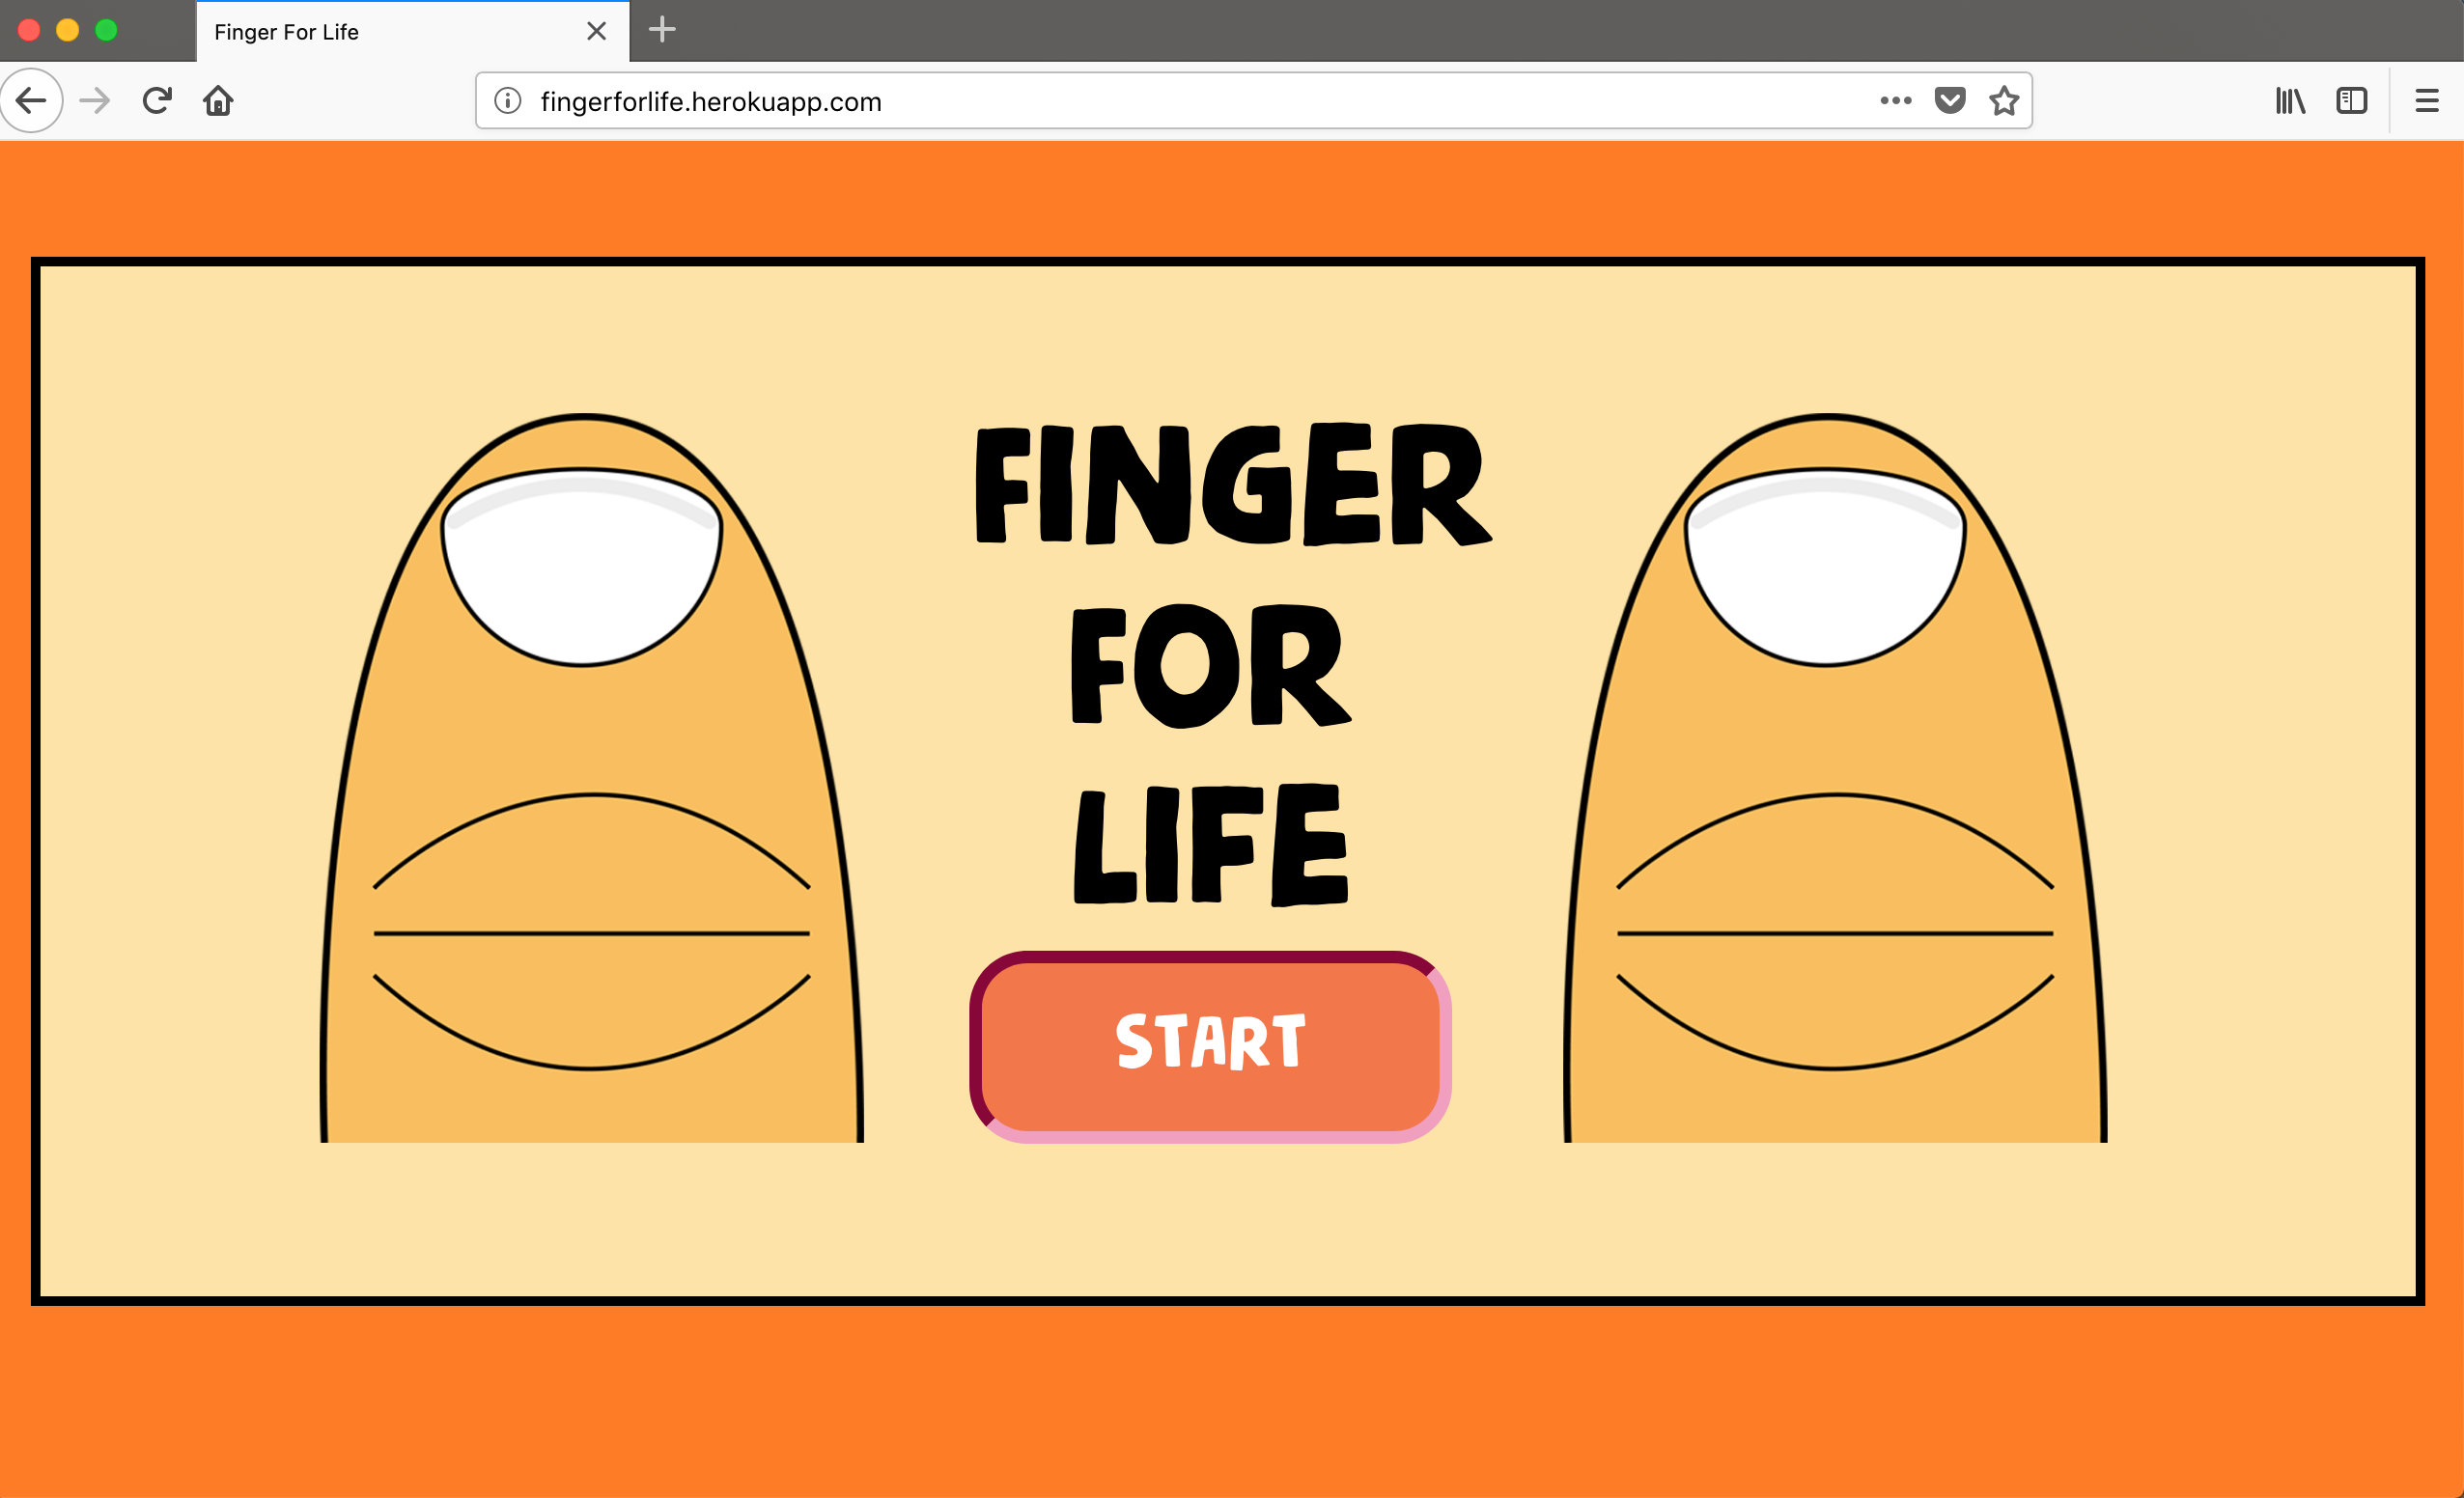
\includegraphics[scale=0.25]{Gambar/realWeb1_home}
	\caption{Halaman \textit{Home}}
	\label{fig:realWeb1_home}
\end{figure}

	\textbf{Smartphone} \\
	Halaman \textit{home} pada \textit{smartphone} digunakan pengguna untuk memulai permainan. Pada halaman ini terdapat tombol \textit{join} yang berfungsi untuk meminta akses masuk kedalam permainan. Apabila pengguna menekan tombol tersebut, maka pengguna akan diarahkan kehalaman selanjutnya. Tangkapan layar dari halaman \textit{home} pada \textit{smartphone} dapat dilihat pada gambar \ref{fig:realPhone1_home}.
	
	\begin{figure}[H]
		\centering
		
\includegraphics[scale=0.2]{Gambar/realPhone1_home}
		\caption{Halaman \textit{Home}}
		\label{fig:realPhone1_home}
	\end{figure}

	\item \textbf{Halaman permintaan bergabung}\\
	\textbf{PC} \\
	Halaman \textit{sync} pada \textit{PC} berguna untuk proses sinkronisasi antara \textit{PC} dan \textit{smartphone}. Halaman ini menyediakan kode \textit{room} yang harus dikirimkan oleh pengguna melalui \textit{smartphone}. Apabila kode yang dikirimkan pengguna sesuai, maka pengguna akan bergabung kedalam \textit{room} permainan. Apabila kode tidak sesuai, maka pengguna tidak bisa bergabung kedalam \textit{room} permainan. Tangkapan layar dari halaman \textit{sync} pada \textit{PC} dapat dilihat pada gambar \ref{fig:realWeb2_sync}.
	
	\begin{figure}[H]
		\centering
		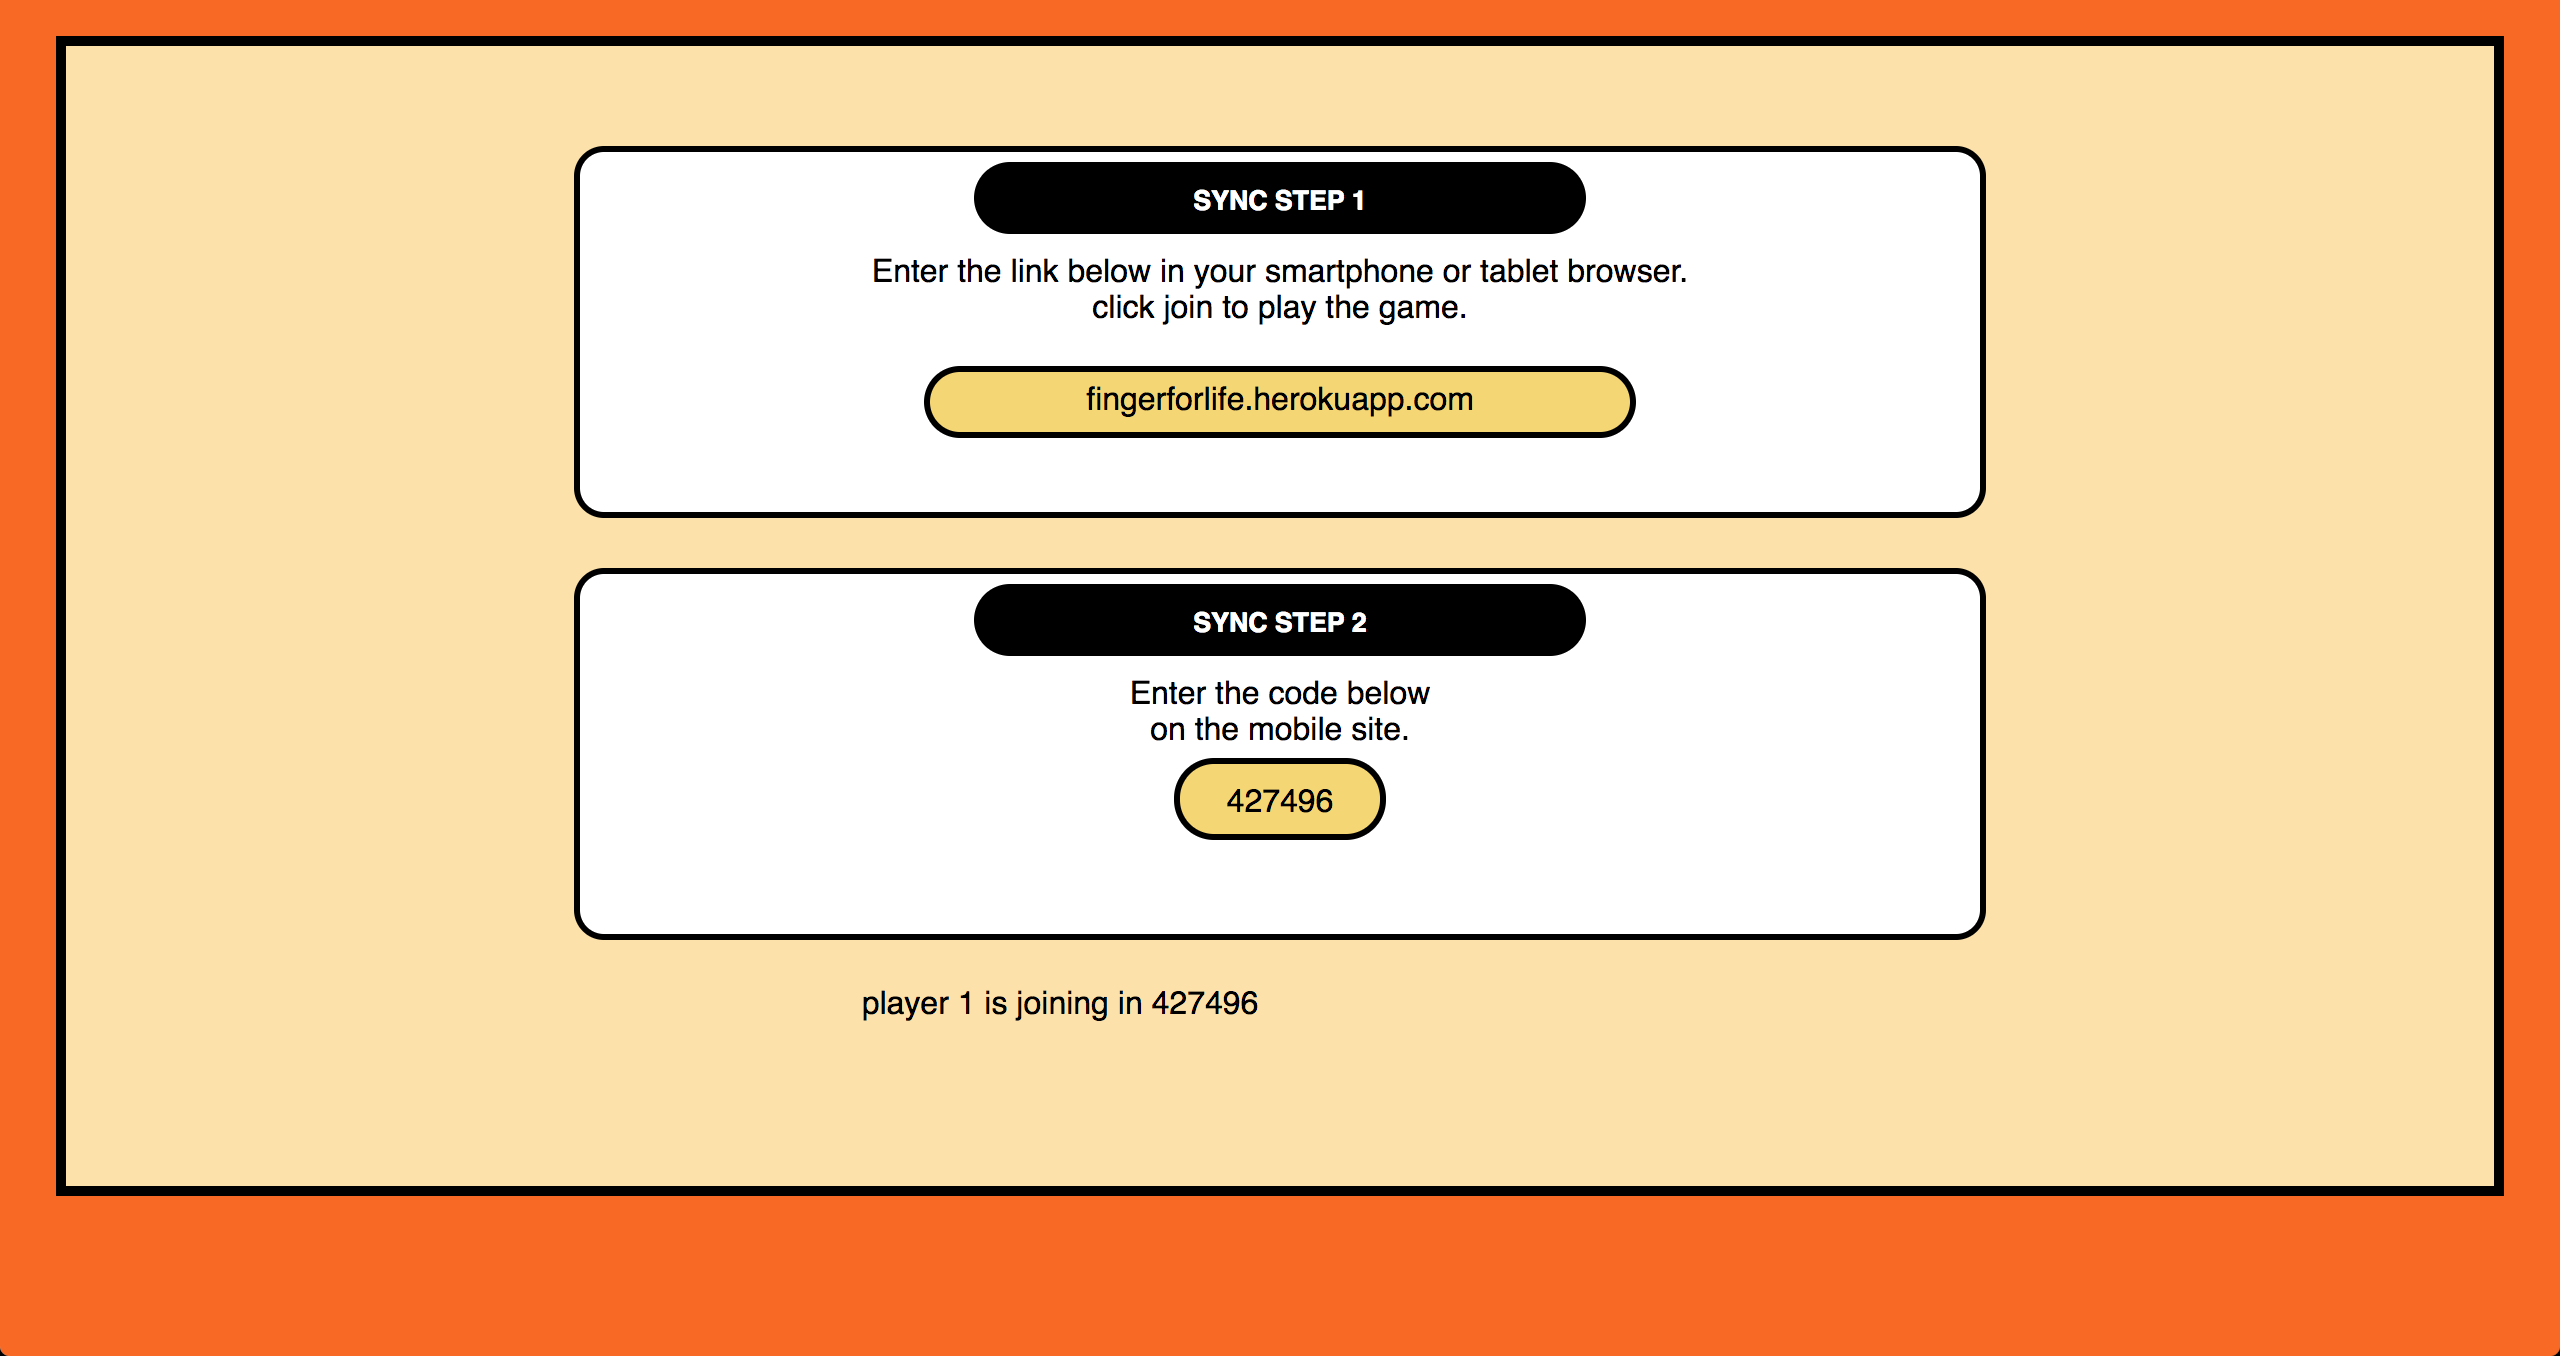
\includegraphics[scale=0.25]{Gambar/realWeb2_sync}
		\caption{Halaman \textit{Home}}
		\label{fig:realWeb2_sync}
	\end{figure}
	
	
	\textbf{Smartphone} \\
	Halaman \textit{sync} pada \textit{smarpthone} berguna untuk proses sinkronisasi antara \textit{PC} dan \textit{smartphone}. Pengguna dapat mengisi kolom dengan kode yang didapatkan dari halaman web pada \textit{PC}, kemudian menekan tombol \textit{Send}. Apabila kode yang dikirimkan sesuai, maka akan muncul teks yang menunjukan berhasil bergabung kedalam \textit{room}. Apabila tidak sesuai, maka akan muncul teks yang menunjukan tidak berhasil bergabung kedalam \textit{room}. Tangkapan layar dari halaman \textit{sync} pada \textit{PC} dapat dilihat pada gambar \ref{fig:realPhone2_sync}.
	
	\begin{figure}[H]
		\centering
		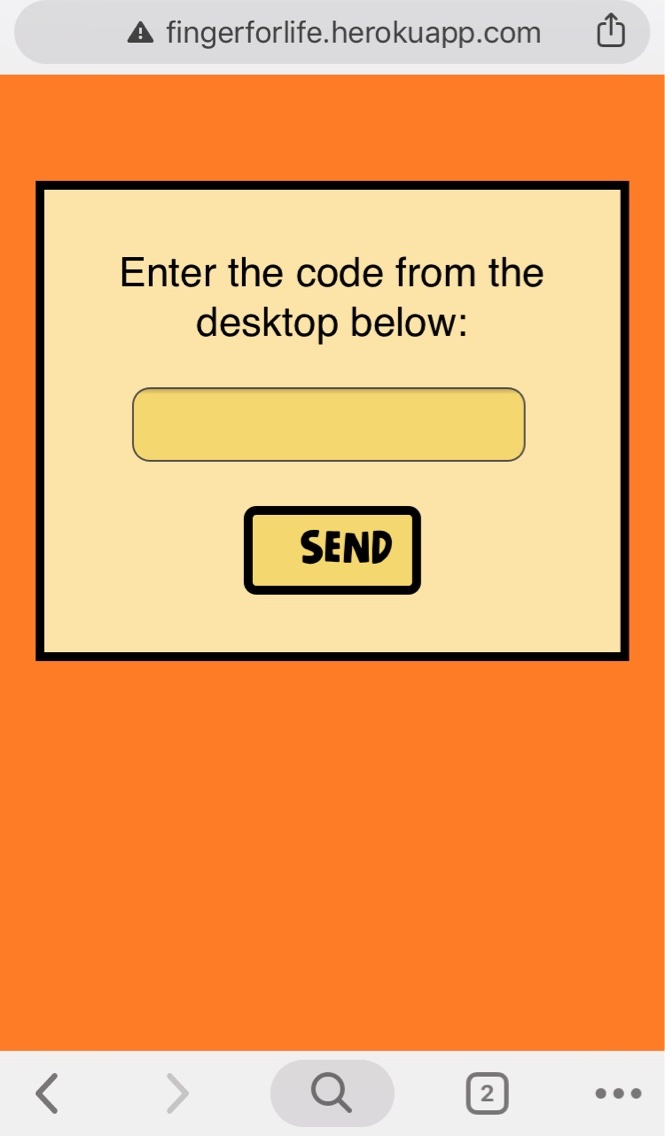
\includegraphics[scale=0.2]{Gambar/realPhone2_sync}
		\caption{Halaman \textit{Home}}
		\label{fig:realPhone2_sync}
	\end{figure}
	
	\item \textbf{Halaman Pemilihan Karakter} \\
	\textbf{PC} \\
	Halaman pemilihan karakter pada \textit{PC} akan menampilkan dua karakter yang telah dipilih oleh kedua pemain. Jika pemain menekan karakter yang terdapat pada halaman \textit{smartphone}, maka karakter tersebut akan ditampilkan. Jika pemain belum menekan karakter yang tersedia, maka halaman pada \textit{PC} tidak akan menampilkan karakter. Tangkapan layar dari halaman pemilihan karakter pada \textit{PC} dapat dilihat pada gambar \ref{fig:realWeb3_char}.
	
	\begin{figure}[H]
		\centering
		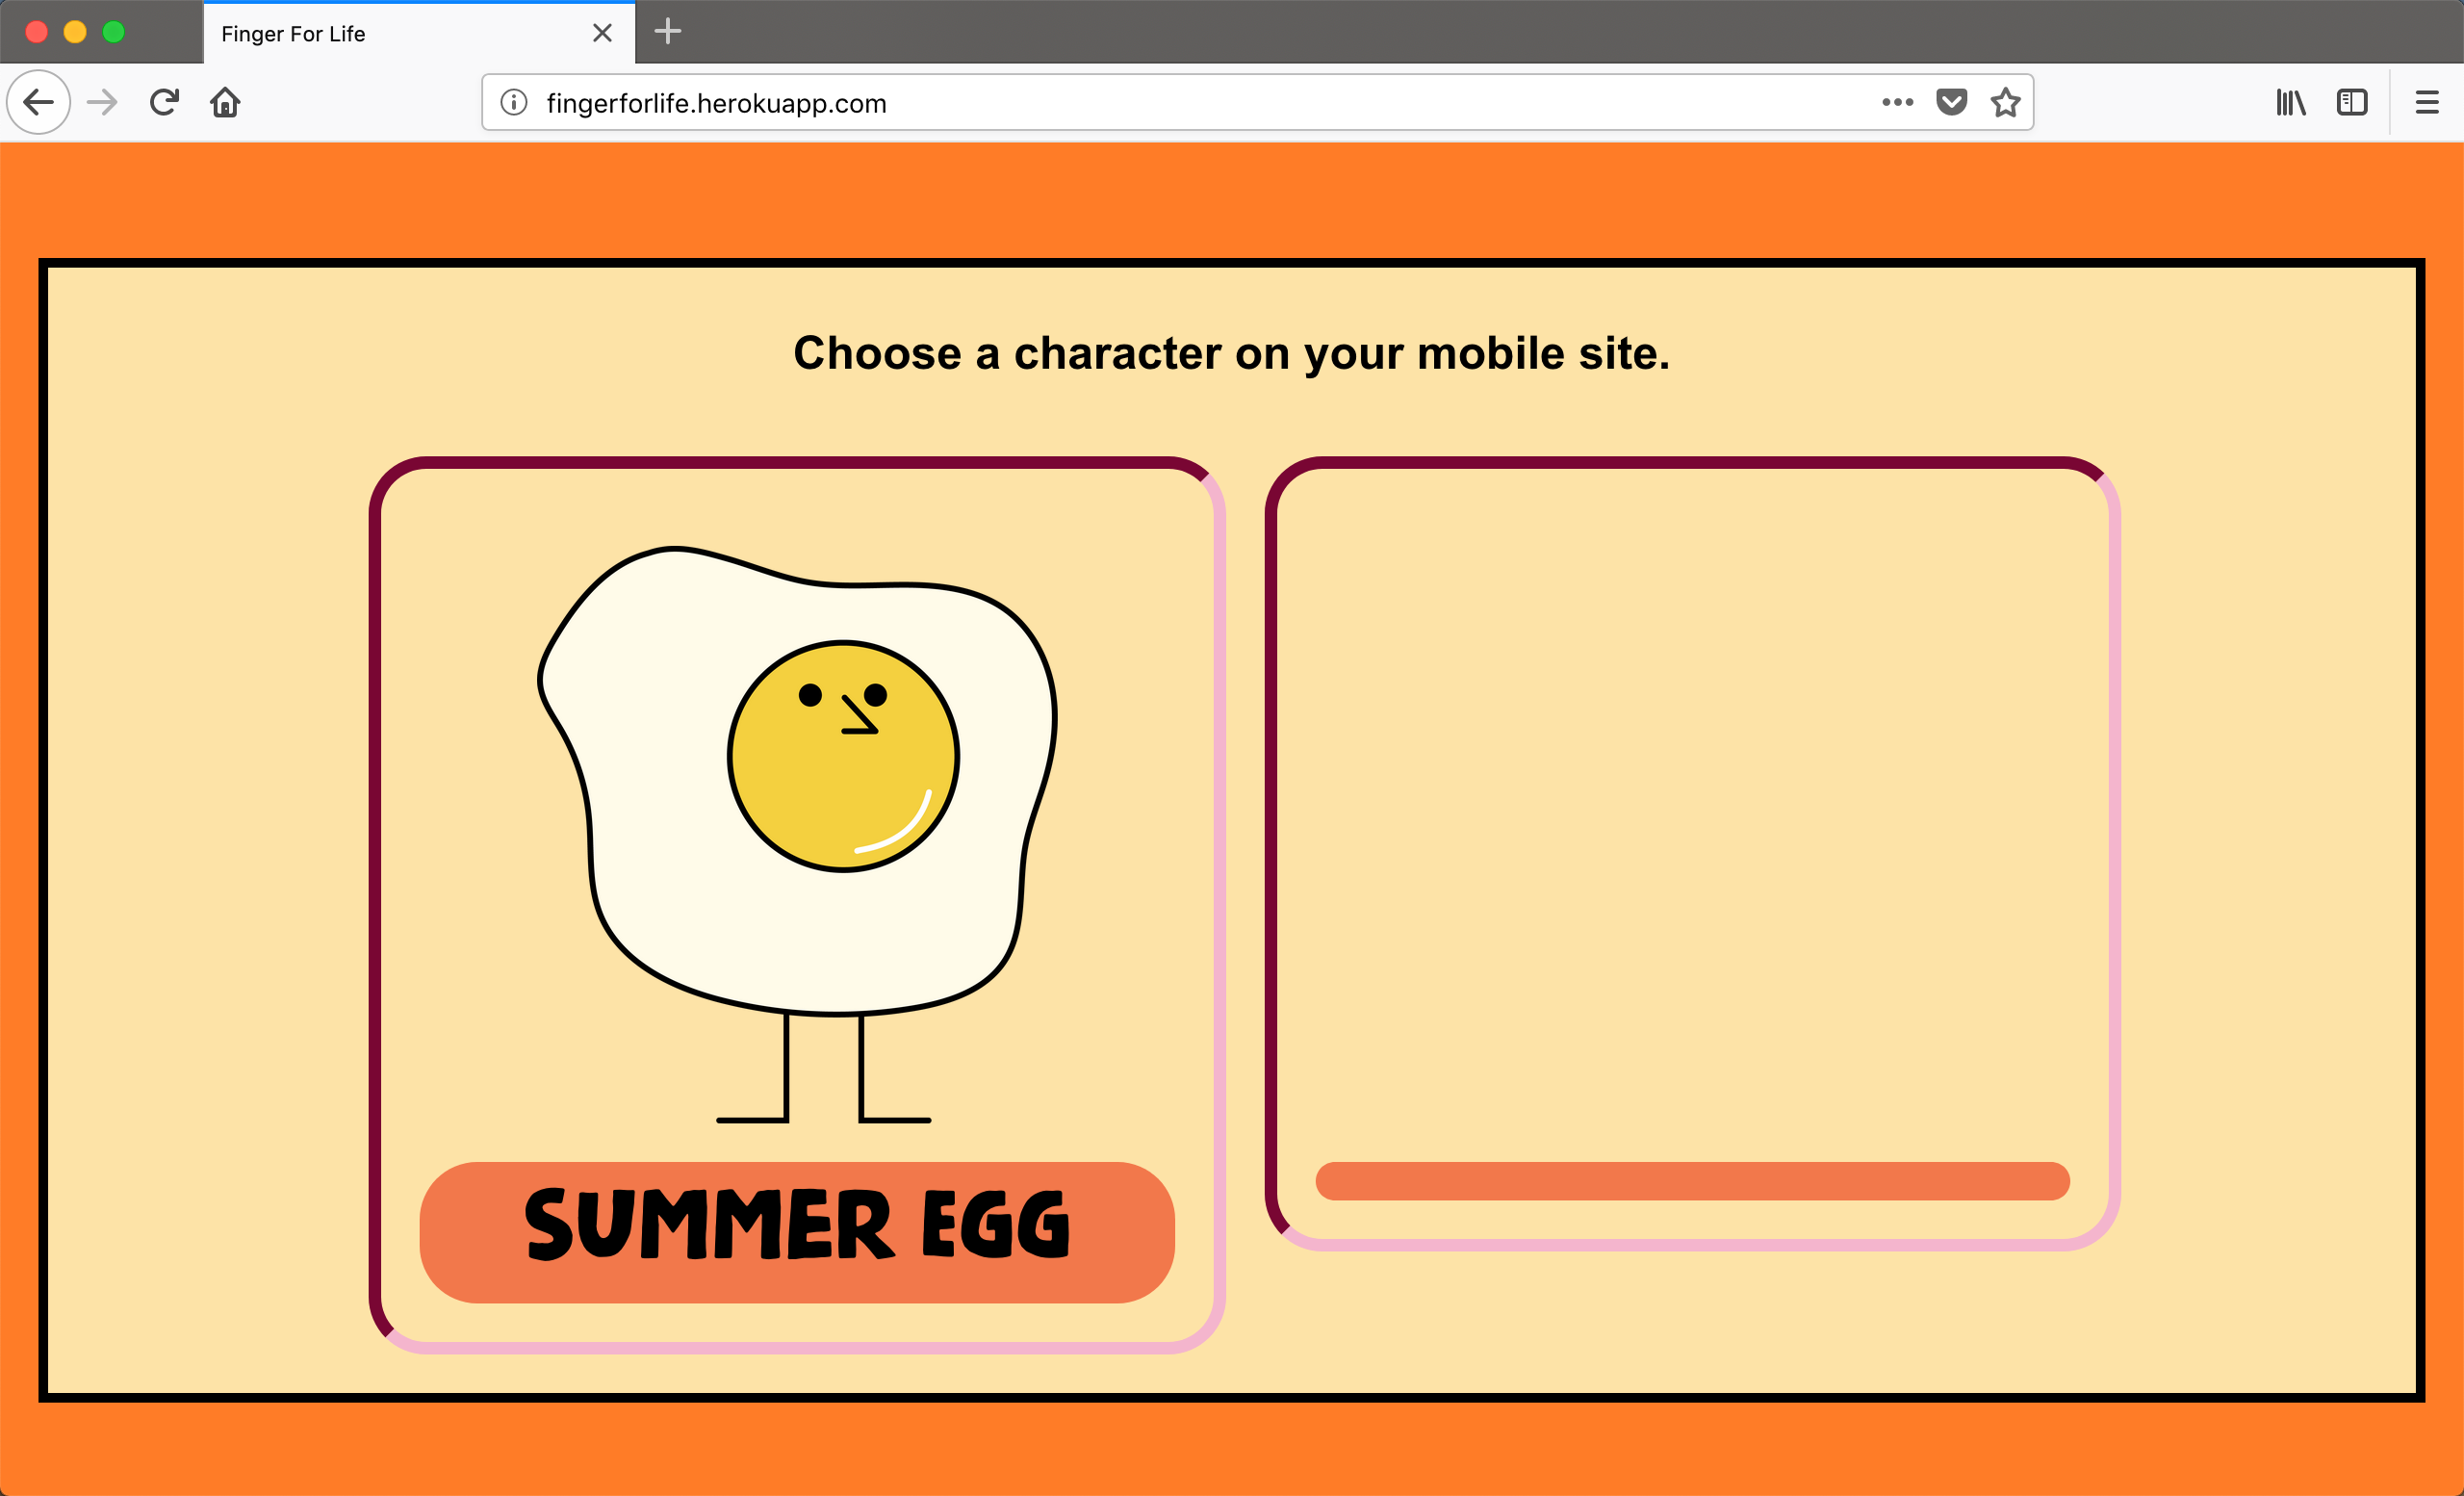
\includegraphics[scale=0.25]{Gambar/realWeb3_char}
		\caption{Halaman \textit{Home}}
		\label{fig:realWeb3_char}
	\end{figure}
	
	\textbf{Smartphone} \\
	Halaman pemilihan karakter pada \textit{smartphone} akan menampilkan daftar karakter permainan Finger For Life. Pemain dapat memilih satu karakter yang ditampilkan, kemudia menekan tombol \textit{choose} untuk menetapkan karakter tersebut. Karakter yang telah ditetapkan akan dapat dimainkan saat permainan dimulai. Apabila kedua pemain telah menetapkan karakter, maka halaman akan berganti kehalaman selanjutnya. Tangkapan layar dari halaman pemilihan karakter pada \textit{smartphone} dapat dilihat pada gambar \ref{fig:realPhone3_char}.
	
	\begin{figure}[H]
		\centering
		
\includegraphics[scale=0.2]{Gambar/realPhone3_char}
		\caption{Halaman \textit{Home}}
		\label{fig:realPhone3_char}
	\end{figure}
	
	\item \textbf{Halaman Permainan} \\
	\textbf{PC} \\
	Halaman ini menampilkan lintasan lari dan kedua karakter yang dapat dimainkan. Karakter pada layar dapat bergerak melalui lintasan lari apabila pemain menekan tombol yang ada pada halaman \textit{smartphone}. Tangkapan layar dari halaman \textit{gameplay} pada \textit{PC} dapat dilihat pada gambar \ref{fig:realWeb4_game}.
	
	\begin{figure}[H]
		\centering
		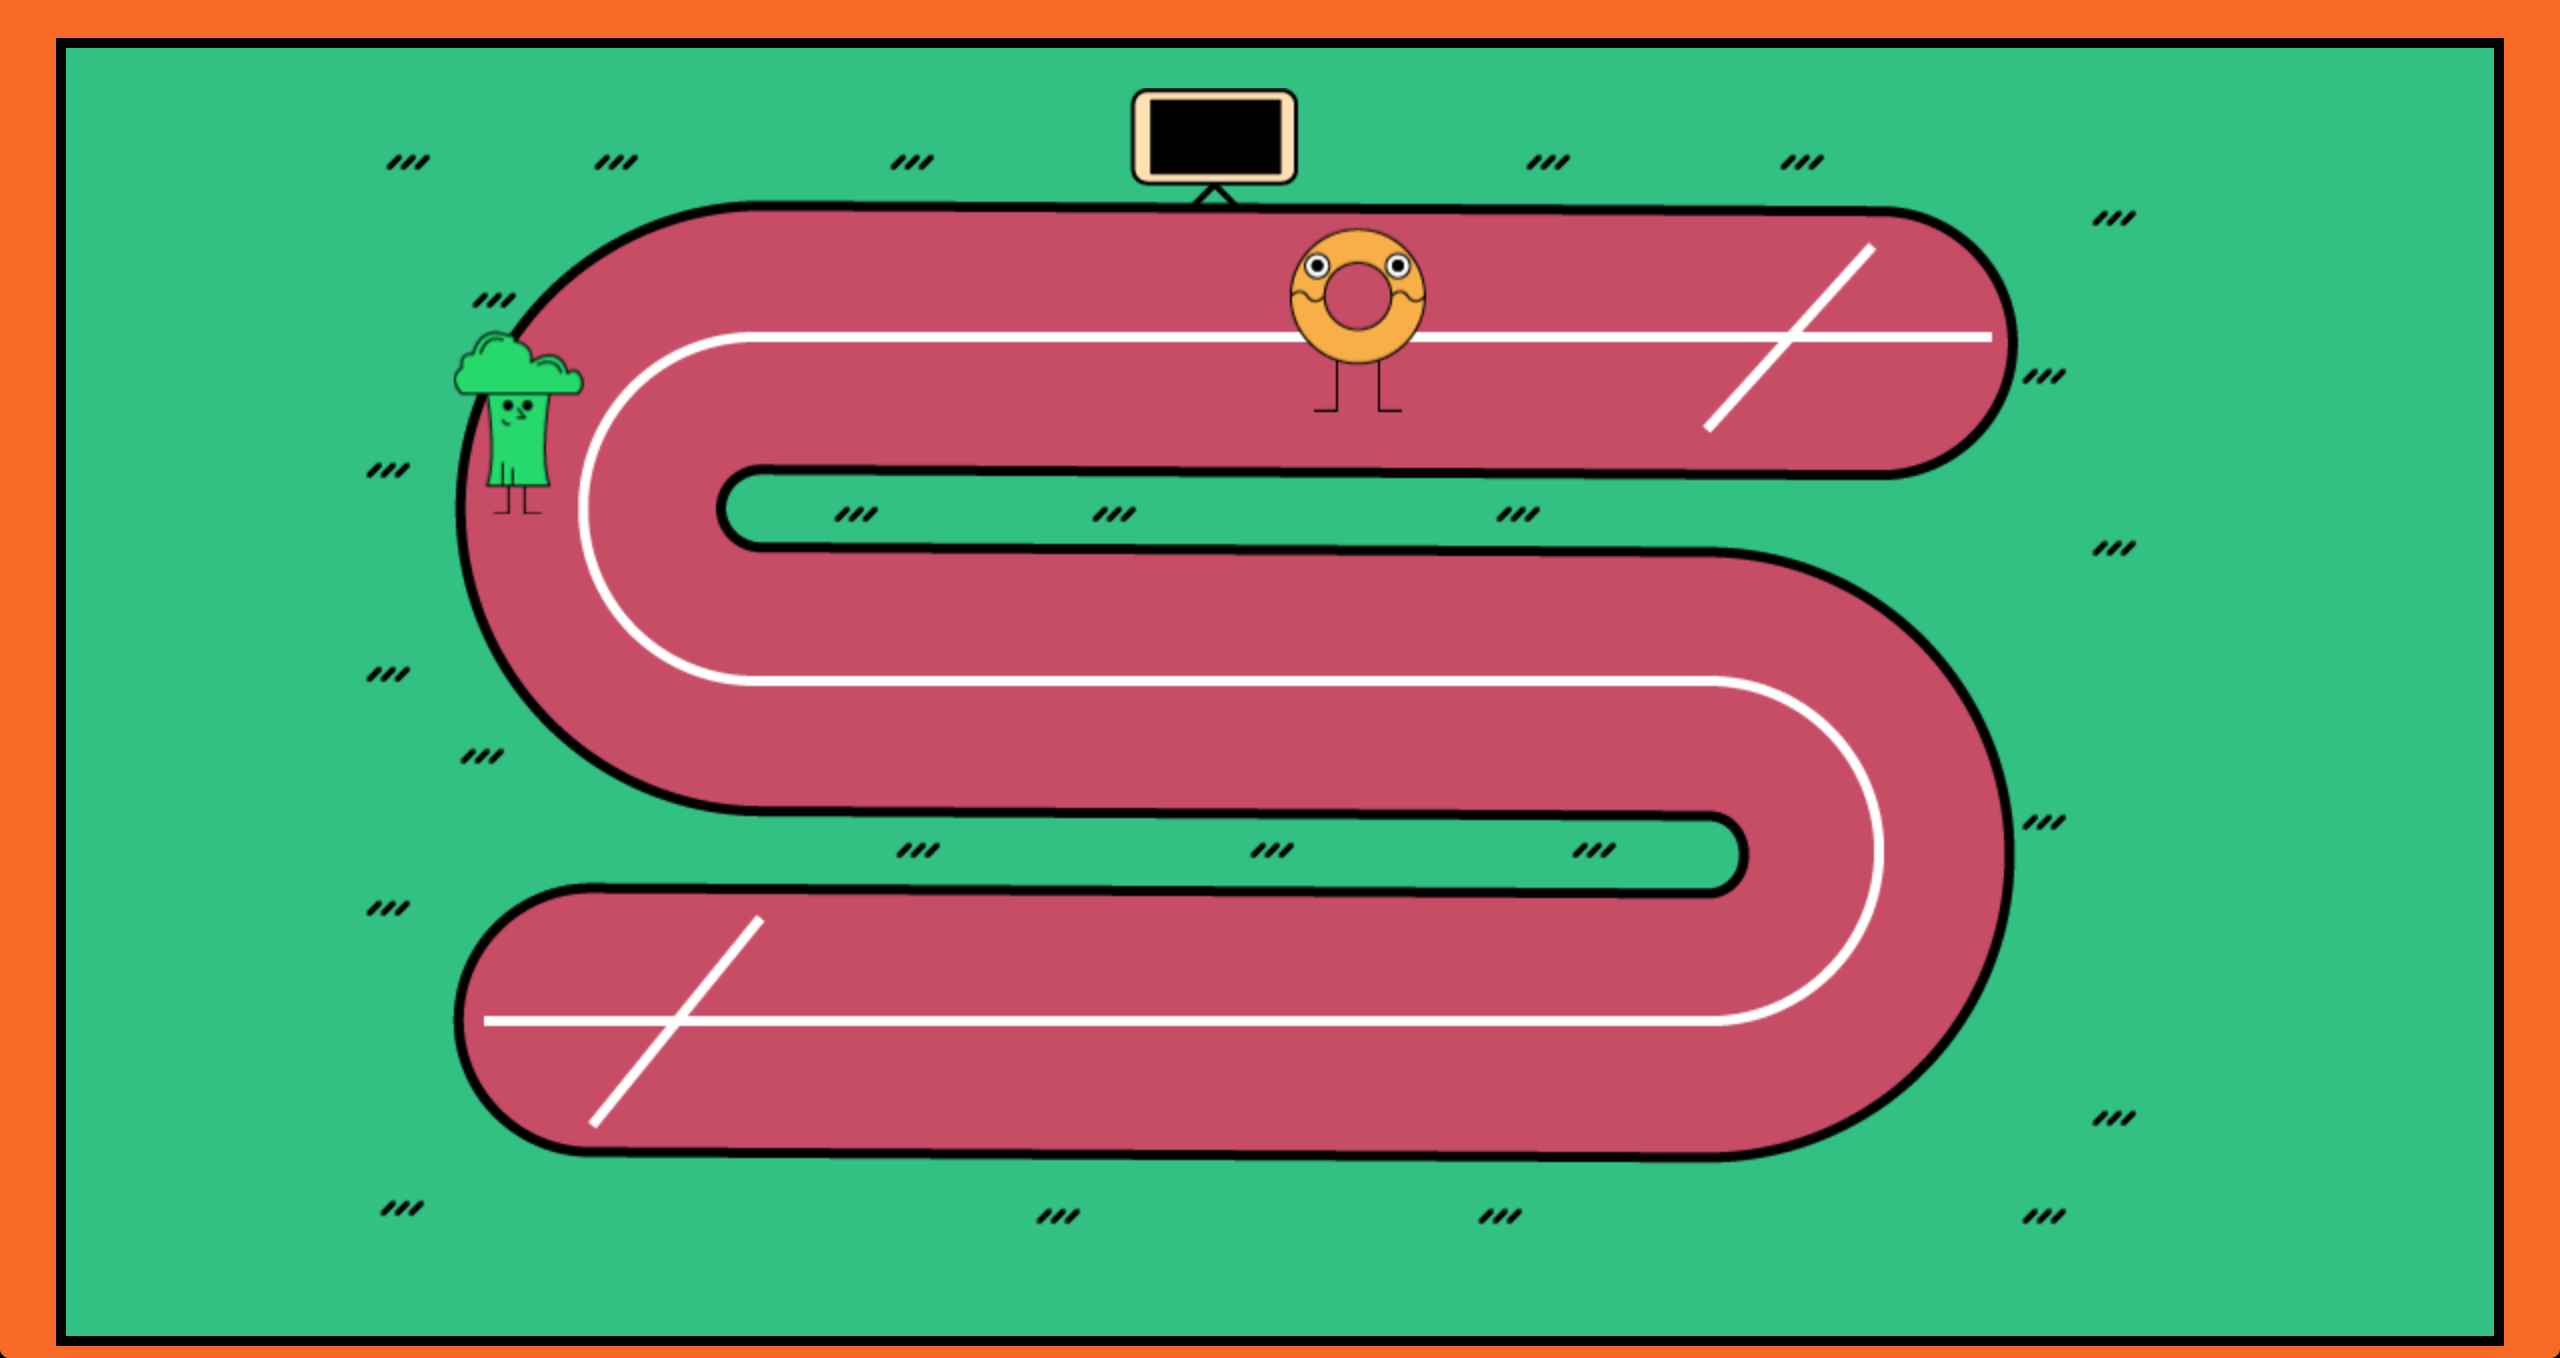
\includegraphics[scale=0.25]{Gambar/realWeb4_game}
		\caption{Halaman \textit{Home}}
		\label{fig:realWeb4_game}
	\end{figure}
	
	\textbf{Smartphone} \\
	Halaman ini menampilkan tombol telapak kaki yang dapat ditekan oleh pemain. Tombol tersebut berfungsi untuk menggerakan karakter miliknya yang ditampilkan dihalaman \textit{PC}. Pemain yang pertama kali menggerakan karakter hingga mencapai garis akhir menjadi pemenang, dan halaman akan berganti kehalaman selanjutnya. Tangkapan layar dari halaman \textit{gameplay} pada \textit{smartphone} dapat dilihat pada gambar \ref{fig:realPhone4_game}.
	
	\begin{figure}[H]
		\centering
		
\includegraphics[scale=0.2]{Gambar/realPhone4_game}
		\caption{Halaman \textit{Home}}
		\label{fig:realPhone4_game}
	\end{figure}
	
	
	\item \textbf{Halaman Permainan Berakhir} \\
	\textbf{PC} \\
	Halaman ini menampilkan pemain yang memenangkan permainan. Pemenang pertama akan ditampilkan dipodium posisi atas, sedangkan pemenang kedua akan ditampilkan dipodium posisi bawah. Pemain dapat menekan tombol \textit{exit} untuk keluar dari permainan. Tangkapan layar dari halaman \textit{game over} pada \textit{PC} dapat dilihat pada gambar \ref{fig:realWeb5_over}.
	
	\begin{figure}[H]
		\centering
		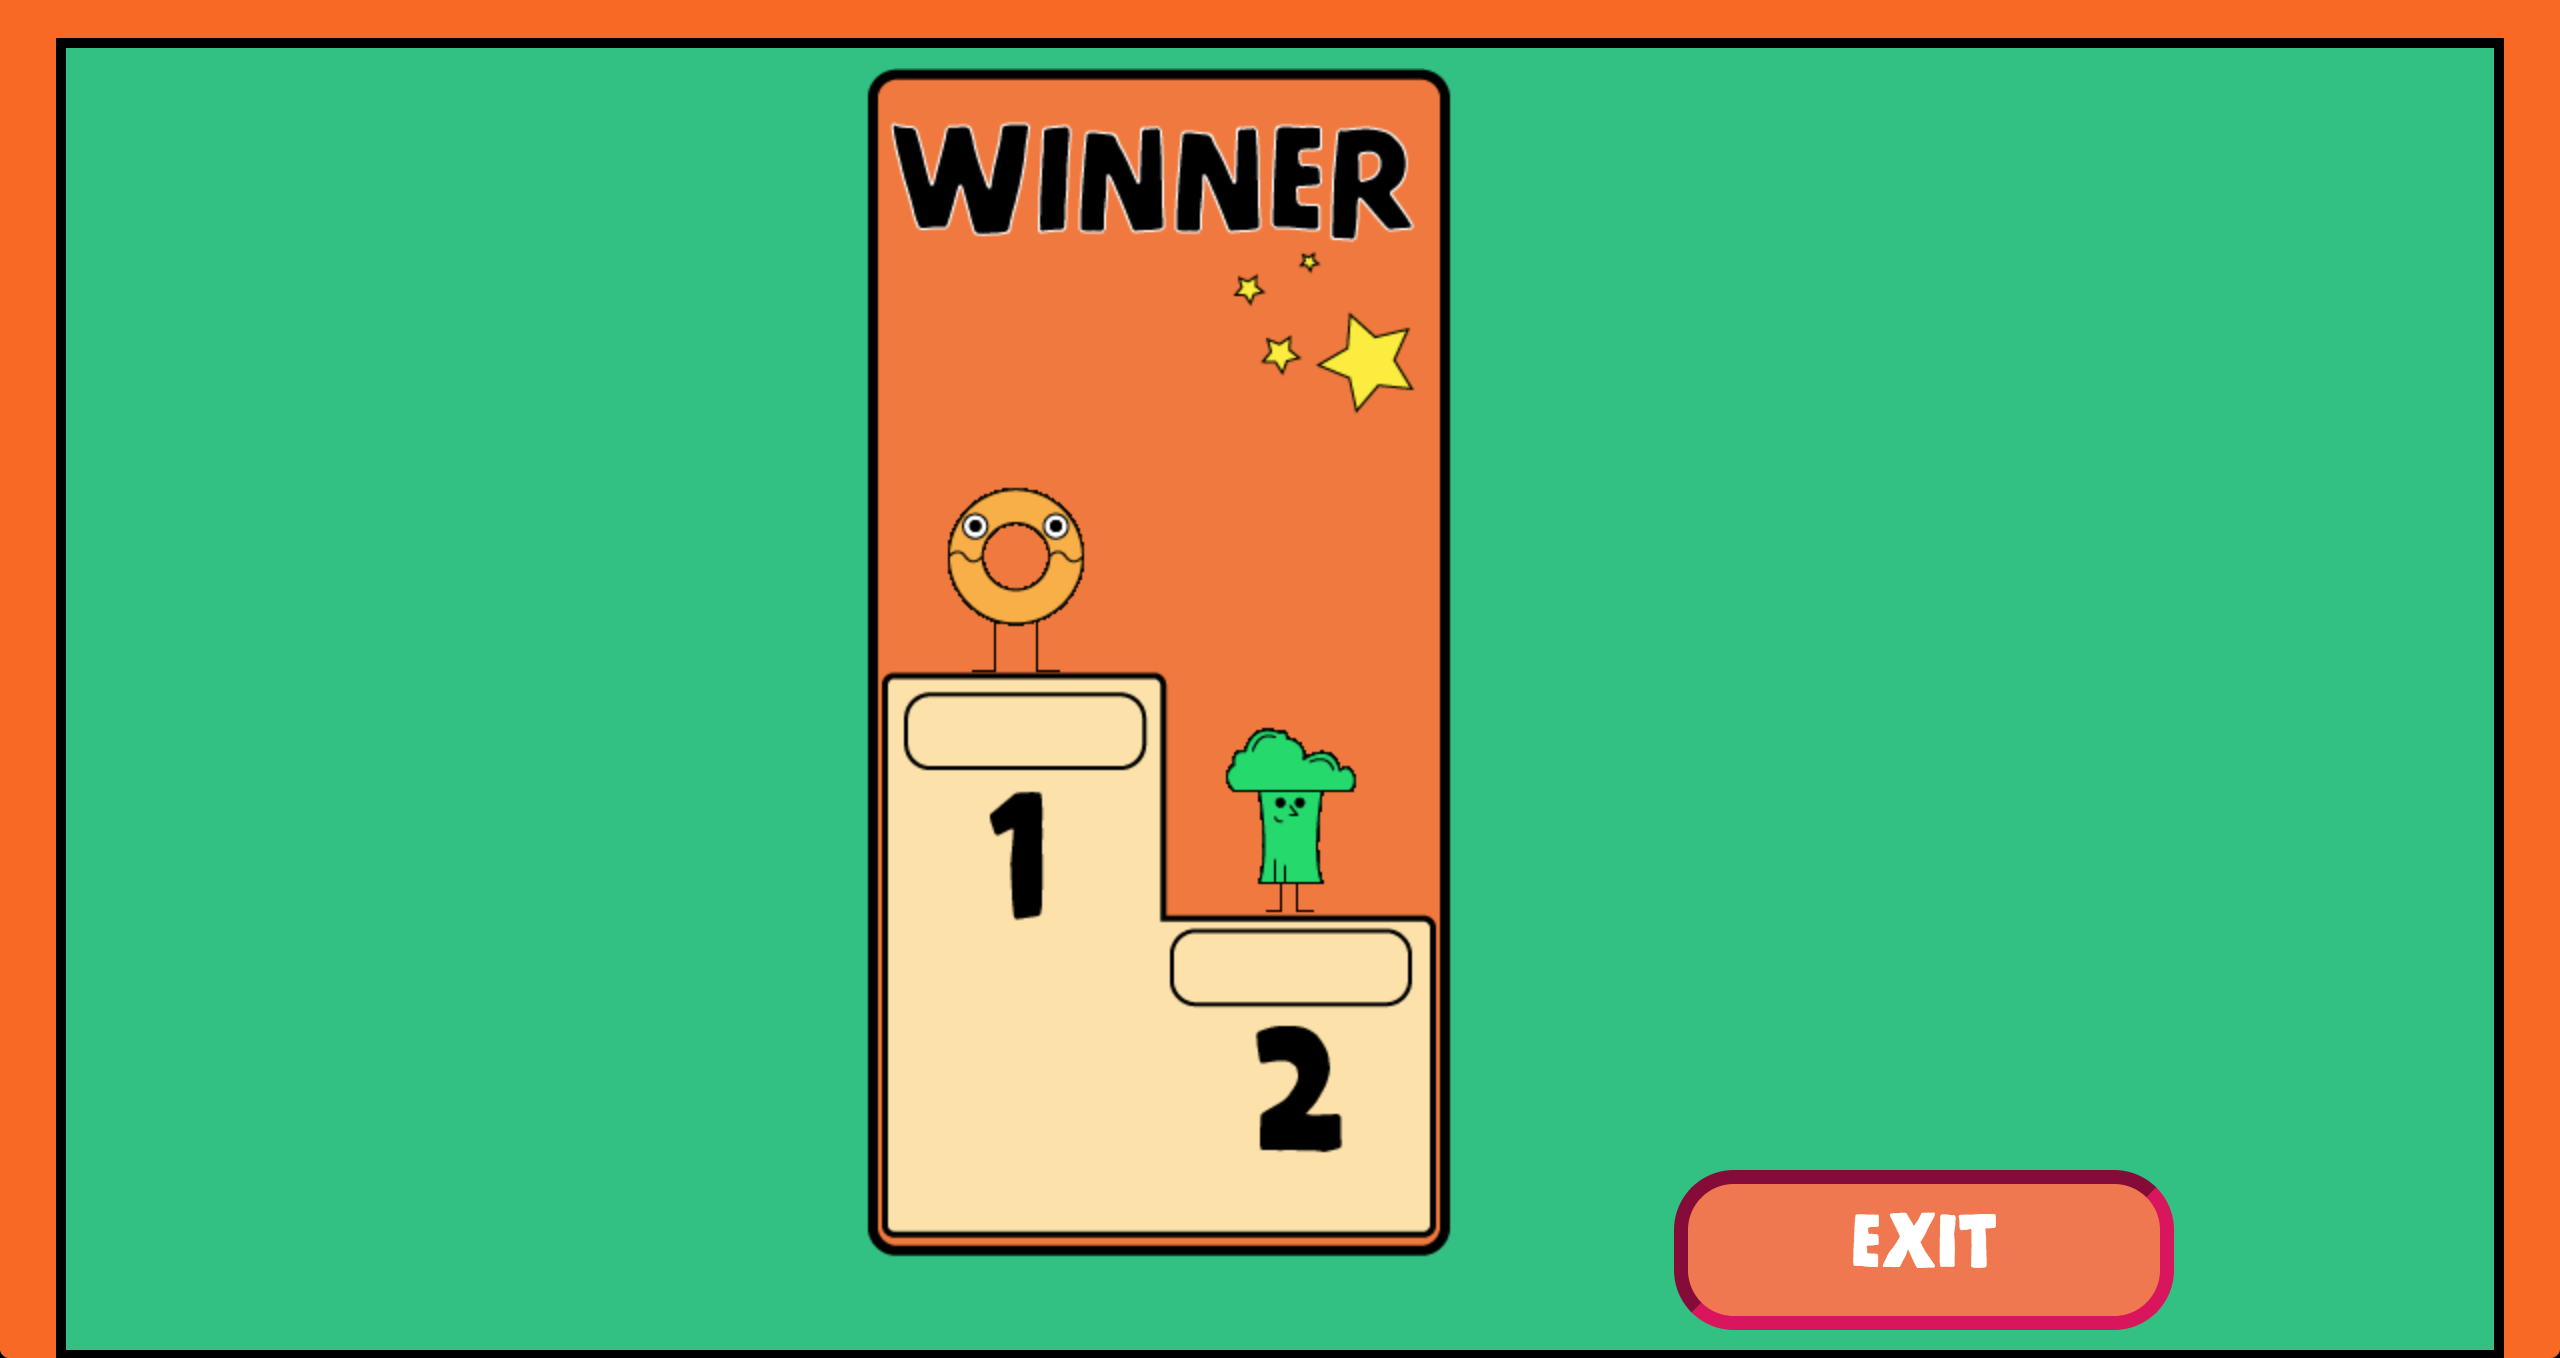
\includegraphics[scale=0.25]{Gambar/realWeb5_over}
		\caption{Halaman \textit{Home}}
		\label{fig:realWeb5_over}
	\end{figure}

	\textbf{Smartphone} \\
	Halaman ini menampilkan teks yang menunjukan posisi pemenang. Pemenang pertama akan ditampilkan teks yang menunjukan posisi pertama, sedangkan pemenang kedua akan ditampilkan teks yang menunjukan posisi kedua. Tangkapan layar dari halaman \textit{game over} pada \textit{smartphone} dapat dilihat pada gambar \ref{fig:realPhone5_over}.
	\begin{figure}[H]
		\centering
		
\includegraphics[scale=0.2]{Gambar/realPhone5_over}
		\caption{Halaman \textit{Home}}
		\label{fig:realPhone5_over}
	\end{figure}

\end{enumerate}


\section{Pengujian}

\subsection{Pengujian Fungsional}
\label{subsec:fungsional}

Pengujian fungsional dilakukan untuk mengetahui kesesuaian reaksi perangkat lunak dengan reaksi yang diharapkan berdasarkan aksi pengguna terhadap perangkat lunak. Pada saat pengujian fungsional dilakukan, penulis menemukan beberapa masalah yang muncul pada program aplikasi. Masalah tersebut muncul pada beberapa tahapan saat program dijalankan. Berdasarkan masalah-masalah yang ditemukan, penulis juga mendapatkan solusi atas masalah yang ada. Berikut akan dijelaskan beberapa masalah yang ditemukan, beserta proses memecahkan masalah yang telah dilakukan.

\begin{enumerate}
	\item \textbf{Halaman \textit{home}}
	\begin{itemize}
		\item \textbf{Masalah:} \\
		Tampilan home pada smartphone terkadang muncul gambar jari. Masalah ini ditemukan pada \textit{smartphone} dengan resolusi layar yang berbeda-beda. Apabila ada \textit{smartphone} dengan resolusi lebih besar dibanding yang lainnya, maka gambar jari muncul dilayar.
		
		\item \textbf{Solusi:} \\
		Solusi dari masalah ini adalah dengan menggunakan fitur dari CSS yaitu \textit{@media querry}. Fitur ini dapat mengatur pada resolusi berapakah suatu elemen ditampilkan kelayar. Berikut merupakan potongan kode solusi dari masalah ini.
		
\begin{lstlisting}[caption={Fitur CSS \textit{@media querry}}, label={lst:mediaQuerry},captionpos=b]
@media (max-width:1260px){
	#left, #right, #startButton{
		display: none;
		float: none;
	}
			
	#joinButton{
		visibility: visible;
		width: 85%;
	}
}
\end{lstlisting}
	\end{itemize}

	\item \textbf{Halaman permintaan bergabung}
	\begin{itemize}
		\item \textbf{Masalah:} \\
		Pada saat kedua pemain menyelesaikan permainan dan menekan tombol \textit{exit}, kemudian kedua pemain akan mengulang permainan dengan menuju ke halaman permintaan bergabung. Pada tahap ini, salah satu pemain tidak dapat bergabung kedalam \textit{room}. \\
		
		\textit{Error} ini terjadi akibat penggunaan elemen jQuery pada halaman permintaan bergabung, yaitu elemen \textit{.submit()}. Pada saat pemain akan bermain kedua kalinya dan sampai dihalaman permintaan bergabung, elemen \textit{submit()} akan mengirimkan kode room lebih dari satu kali. Dengan begitu, \textit{server} akan mengira bahwa ada dua pemain yang sudah bergabung, sehingga halaman langsung berpindah kehalaman selanjutnya. Padahal pemain kedua belum mengisi kode \textit{room} dan belum mengirimkan ke \textit{server}.
		
		\item \textbf{Solusi:} \\
		Solusi dari masalah ini adalah dengan menghilangkan elemen \textit{submit()}, kemudian diganti dengan menggunakan Socket.io untuk memancarkan \textit{event} pada saat tombol \textit{send} ditekan. Berikut merupakan potongan kode dari solusi masalah ini.
		
\begin{lstlisting}[caption={Proses memancarkan \textit{event}}, label={lst:emitEvent},captionpos=b]
function requestToJoin(){
	socket.emit('requestToJoin', {
		id: socket.id,
		room: $('#code').val()
	});
}
\end{lstlisting}	
	\end{itemize}
	
	\item \textbf{Halaman pemilihan karakter}
	\begin{itemize}
		\item \textbf{Masalah:} \\
		Pada saat salah satu pemain menekan tombol \textit{choose} dua kali, halaman langsung pindah kehalaman \textit{gameplay} disaat pemain kedua belum memilih karakter. \\
		
		\textit{Error} terjadi karena pada saat pemain menekan tombol choose, seluruh data langsung dikirimkan ke \textit{server} sehingga \textit{server} menangkap sudah ada satu pemain yang berhasil mengirimkan data karakter. Apabila ditekan dua kali, maka akan dianggap sudah ada dua pemain yang mengirimkan data karakter. Dengan begitu halaman pun berpindah.
		
		\item \textbf{Solusi:} \\
		Solusi untuk masalah ini adalah dengan menggunakan JavaScript untuk menangani tombol \textit{choose}, sehingga pemain tidak dapat mengirimkan data apabila belum memilih karakter. Setelah itu, tombol \textit{choose}  milik pemain yang telah memilih karakter akan dinonaktifkan, sehingga tidak dapat ditekan dua kali. Berikut merupakan potongan kode dari solusi masalah ini:
		
\begin{lstlisting}[caption={Proses menangani tombol \textit{choose}}, label={lst:tombolChoose},captionpos=b]
var valButton = $('input[name="radioChar"]:checked').val();
	if (valButton === undefined) {
	alert("You have not choose a character.");
}
else{
	socket.emit('sendingChar', {
	val: valButton,
	id: socket.id,
	marker: 1
});
document.getElementById("nextButton").disabled = true;
}
\end{lstlisting}
	\end{itemize}

	\item \textbf{Halaman pemilihan karakter}
	\begin{itemize}
		\item \textbf{Masalah:} \\
		Pada saat memilih karakter, setelah ditekan karakternya pada \textit{smartphone}, karakter tidak muncul dilayar \textit{PC}.\\
		
		\textit{Error} ini terjadi karena adanya kesalahan pengiriman data pada saat proses bergabung kedalam \textit{room}. Yang masuk kedalam \textit{room} hanya satu pemain saja, sedangkan pemain kedua tidak mengirimkan data kepada \textit{server} sehingga tidak masuk kedalam \textit{room}.
		
		\item \textbf{Solusi:} \\
		Solusi dari masalah ini adalah dengan menggunakan JavaScript, untuk menangani proses permintaan bergabung agar kedua pemain dapat masuk kedalam room. Berikut merupakan potongan kode dari solusi masalah ini:
		
\begin{lstlisting}[caption={Proses menangani memancarkan \textit{event}}, label={lst:submitEvent},captionpos=b]
function requestToJoin(){
	socket.emit('requestToJoin', {
		id: socket.id,
		room: $('#code').val()
	});
}
\end{lstlisting}
	\end{itemize}
\end{enumerate}

Pengujian fungsional yang dilakukan terbagi menjadi dua, yaitu pengujian fungsional pada \textit{PC} dan pada \textit{smartphone}.

\textbf{PC} \\
\begin{table}[H]
	\centering
	\caption{Tabel Pengujian Fungsional pada \textit{PC}}
	\begin{tabular}{|p{0.35cm}| p{3.5cm}| p{7cm}| p{2.5cm}|} \hline
		No. & Aksi Pengguna & Reaksi yang diharapkan & Reaksi perangkat lunak \\ \hline
		1 & Pengguna menjalankan aplikasi & Halaman \textit{home} akan ditampilkan & sesuai \\ \hline
		2 & Pengguna menekan tombol \textit{start} & Halaman akan diarahkan menuju halaman pemintaan bergabung & sesuai \\ \hline
		3 & Pengguna melakukan proses sinkronisasi \textit{PC} dan \textit{smartphone}. & Jika pemain pertama berhasil bergabung kedalam \textit{room}, maka pada layar \textit{PC} akan muncul pesan "Player 1 has join the room" & sesuai \\ \hline
		&  & Jika pemain kedua berhasil bergabung kedalam \textit{room}, maka pada layar \textit{PC} akan muncul pesan "Player 2 has join the room", kemudian halaman langsung diarahkan menuju halaman pemilihan karakter & sesuai \\ \hline
		4 & Pengguna melakukan proses pemilihan karakter & Jika para pemain memilih karakter, maka kedua karakter yang dipilih akan ditampilkan kelayar \textit{PC} & sesuai \\ \hline
		&  & Jika para pemain telah menetapkan karakter yang dipilih, maka halaman akan diarahkan menuju halaman permainan & sesuai \\ \hline
		5 & Pengguna mulai memainkan permainan & Karakter milik pemain bergerak melalui lintasan lari selama permainan dan akan diarahkan kehalaman permainan berakhir apabila ada yang menyentuh garis akhir lebih dulu & sesuai \\ \hline
		6 & Pengguna menekan tombol \textit{exit} & Permainan berakhir dan halaman diarahkan kembali menuju halaman \textit{home} & sesuai \\ \hline
	\end{tabular}
	\label{table:fungsionalPC}
\end{table} 

\textbf{Smartphone} \\
\begin{table}[H]
	\centering
	\caption{Tabel Pengujian Fungsional pada \textit{smartphone}}
	\begin{tabular}{|p{0.35cm}| p{3.5cm}| p{7cm}| p{2.5cm}|} \hline
		No. & Aksi Pengguna & Reaksi yang diharapkan & Reaksi perangkat lunak \\ \hline
		1 & Penggunan menjalankan aplikasi & Halaman \textit{home} ditampilkan & sesuai \\ \hline 
		2 & Pengguna menekan tombol \textit{join} & Halaman akan diarahkan menuju halaman permintaan bergabung & sesuai \\ \hline
		3 & Pengguna memasukan kode \textit{room} dan menekan tombol \textit{send} & Jika kode \textit{room} sesuai, maka akan muncul pesan "Welcome to the game !" & sesuai \\ \hline
		& & Jika kedua pemain berhasil bergabung, maka halaman akan diarahkan menuju halaman pemilihan karakter & sesuai \\ \hline
		4 & Pengguna menekan karakter pada layar \textit{smartphone} & Karakter yang ditekan akan ditampilkan dilayar \textit{PC} & sesuai \\ \hline
		& & Jika kedua pemain telah memilih karakter, maka halaman akan diarahkan menuju halaman permainan & sesuai \\ \hline
		5 & Pengguna menekan tombol telapak kaki secara berulang selama permainan & Karakter pada layar \textit{PC} akan bergerak & sesuai\\ \hline
		& & Jika ada pemain yang lebih dulu mencapai garis akhir, maka halaman akan diarahkan menuju halaman permainan berakhir & sesuai \\ \hline
		6 & Pengguna mengakhiri permainan & Halaman diarahkan kembali menuju halaman \textit{home} & sesuai \\ \hline
	\end{tabular}
	\label{table:fungsionalSmartphone}
\end{table}
\subsection{Pengujian Eksperimental}
Pengujian eksperimental dilakukan terhadap beberapa responden dengan \textit{smartphone} dan \textit{PC} yang berbeda-beda. Setiap responden diminta untuk mengakses URL yang diberikan melalui \textit{smartphone} dan \textit{PC} milik masing-masing dan memastikan apakah fungsi dari setiap halaman yang ditampilkan sudah berjalan. Pengujian eksperimental terbagi menjadi dua, yaitu pengujian \textit{cross-platform} dan pengujian \textit{latency}.

\begin{enumerate}
	\item \textbf{Pengujian \textit{Cross-Platform}} \\
	Pengujian \textit{cross-platform} dilakukan terhadap jenis \textit{smartphone} dan jenis \textit{browser} yang berbeda-beda. Pengujian ini dilakukan untuk memastikan setiap fungsi dari setiap halaman yang ditampilkan sudah berjalan diseluruh \textit{platform}. Dari beberapa responden yang sudah melakukan pengujian, didapatkan hasil sebagai berikut:
	
	\begin{enumerate}
		\item \textbf{Pengujian pertama} \\
		Jenis \textit{smartphone} pemain 1: iPhone 7 \\
		Jenis \textit{browser} pemain 1: Safari\\
		Jaringan internet pemain 1: Telkomsel\\
		
		Jenis \textit{smartphone} pemain 2: iPhone 7 Plus\\
		Jenis \textit{browser} pemain 2: Google Chrome\\
		Jaringan internet pemain 2: Telkomsel\\
		
		Jenis \textit{PC}: Macbook 13" mid 2014\\
		Jenis \textit{browser PC}: Google Chrome\\
		Jaringan internet \textit{PC}: Wifi UNPAR9\\
		
		Hasil: Berdasarkan tabel \ref{table:fungsionalPC} dan \ref{table:fungsionalSmartphone} yang ada pada subbab \ref{subsec:fungsional}, seluruh fungsi telah berjalan dengan baik.
		
		\item \textbf{Pengujian kedua} \\
		Jenis \textit{smartphone} pemain 1: Samsung Galaxy S4\\
		Jenis \textit{browser} pemain 1: Google Chrome\\
		Jaringan internet pemain 1: Wifi Megavision\\
		
		Jenis \textit{smartphone} pemain 2: Motorola Moto G (5S Plus)\\
		Jenis \textit{browser} pemain 2: Dolphin Browser\\
		Jaringan internet pemain 2: Wifi Megavision\\
		
		Jenis \textit{PC}: Asus A450L\\
		Jenis \textit{browser PC}: Google Chrome\\
		Jaringan internet \textit{PC}: Wifi Megavision\\
		
		Hasil: Berdasarkan tabel \ref{table:fungsionalPC} dan \ref{table:fungsionalSmartphone} yang ada pada subbab \ref{subsec:fungsional}, seluruh fungsi telah berjalan dengan baik.
		
		\item \textbf{Pengujian ketiga} \\
		Jenis \textit{smartphone} pemain 1: iPhone 7 Plus\\
		Jenis \textit{browser} pemain 1: Google Chrome\\
		Jaringan internet pemain 1: Telkomsel\\
		
		Jenis \textit{smartphone} pemain 2: iPhone 7 Plus\\
		Jenis \textit{browser} pemain 2: Safari\\
		Jaringan internet pemain 2: Telkomsel\\
		
		Jenis \textit{PC}: Asus ROG FX\\
		Jenis \textit{browser PC}: Google Chrome\\
		Jaringan internet \textit{PC}: Wifi UNPAR9\\
		
		Hasil: Berdasarkan tabel \ref{table:fungsionalPC} dan \ref{table:fungsionalSmartphone} yang ada pada subbab \ref{subsec:fungsional}, seluruh fungsi telah berjalan dengan baik.
		
		\item \textbf{Pengujian keempat} \\
		Jenis \textit{smartphone} pemain 1: iPhone 7\\
		Jenis \textit{browser} pemain 1: Google Chrome\\
		Jaringan internet pemain 1: Telkomsel\\
		
		Jenis \textit{smartphone} pemain 2: Xiaomi mi note 3\\
		Jenis \textit{browser} pemain 2: Google Chrome\\
		Jaringan internet pemain 2: Telkomsel\\
		
		Jenis \textit{PC}: Macbook Pro 13" Mid 2014\\
		Jenis \textit{browser PC}: Google Chrome\\
		Jaringan internet \textit{PC}: Wifi The Kiosk\\
		
		Hasil: Berdasarkan tabel \ref{table:fungsionalPC} dan \ref{table:fungsionalSmartphone} yang ada pada subbab \ref{subsec:fungsional}, seluruh fungsi telah berjalan dengan baik.
		
		\item \textbf{Pengujian kelima} \\
		Jenis \textit{smartphone} pemain 1: Samsung J7 Pro\\
		Jenis \textit{browser} pemain 1: Google Chrome\\
		Jaringan internet pemain 1: Telkomsel\\
		
		Jenis \textit{smartphone} pemain 2: iPhone 7 Plus\\
		Jenis \textit{browser} pemain 2: Google Chrome\\
		Jaringan internet pemain 2: Telkomsel\\
		
		Jenis \textit{PC}: Asus ROG FX\\
		Jenis \textit{browser PC}: Google Chrome\\
		Jaringan internet \textit{PC}: Wifi UNPAR9\\
		
		Hasil: Berdasarkan tabel \ref{table:fungsionalPC} dan \ref{table:fungsionalSmartphone} yang ada pada subbab \ref{subsec:fungsional}, seluruh fungsi telah berjalan dengan baik.
	\end{enumerate}

	Dari beberapa pengujian yang dilakukan, dapat disimpulkan bahwa aplikasi telah berjalan dengan baik di beberapa \textit{platform} yang berbeda.
	
	
	\item \textbf{Pengujian \textit{latency}} \\
	Pengujian ini dilakukan untuk meneliti jumlah \textit{latency} yang dihasilkan dari implementasi Socket.io. Pengujian \textit{latency} yang dilakukan berfokus pada halaman \textit{gameplay}, saat kedua pemain memainkan permainan Finger For Life. \textit{Latency} yang dihitung adalah perbandingan waktu antara pemain menekan tombol kaki pada layar \textit{smartphone} hingga karakter pada layar \textit{PC} bergerak. 
	
	Dari beberapa responden yang melakukan pengujian, didapatkan beberapa hasil seperti berikut:
	
	\begin{enumerate}
		\item \textbf{Pengujian Pertama} \\ 
		Jenis \textit{smartphone} pemain 1: Samsung J7\\
		Jenis \textit{browser} pemain 1: Internet (Default Browser Android)\\
		Jaringan internet pemain 1: Wifi UNPAR2\\
		
		Jenis \textit{smartphone} pemain 2: LG Q6+\\
		Jenis \textit{browser} pemain 2: Google Chrome\\
		Jaringan internet pemain 2: Wifi UNPAR2\\
		
		Jenis \textit{PC}: HP Pavilion G4\\
		Jenis \textit{browser PC} : Mozilla Firefox\\
		Jaringan internet \textit{PC}: Wifi UNPAR2\\
		
		Hasil: Berdasarkan percobaan yang telah dilakukan, jumlah \textit{latency} yang dihasilkan oleh pemain 1 adalah 203 \textit{millisecond}, dan jumlah \textit{latency} yang dihasilkan oleh pemain 2 adalah 203 \textit{millisecond}.
		
		\item \textbf{Pengujian Kedua} \\ 
		Jenis \textit{smartphone} pemain 1: iPhone 7\\
		Jenis \textit{browser} pemain 1: Google Chrome\\
		Jaringan internet pemain 1: Telkomsel\\
		
		Jenis \textit{smartphone} pemain 2: Xiaomi Mi Note 3\\
		Jenis \textit{browser} pemain 2: Google Chrome\\
		Jaringan internet pemain 2: Telkomsel\\
		
		Jenis \textit{PC}: Macbook Pro 13" Mid 2014\\
		Jenis \textit{browser PC} : Google Chrome\\
		Jaringan internet \textit{PC}: Wifi Telkomsel\\
		
		Hasil: Berdasarkan percobaan yang telah dilakukan, jumlah \textit{latency} yang dihasilkan oleh pemain 1 adalah 277 \textit{millisecond}, dan jumlah \textit{latency} yang dihasilkan oleh pemain 2 adalah 298 \textit{millisecond}.
		
		\item \textbf{Pengujian Ketiga} \\ 
		Jenis \textit{smartphone} pemain 1: coolpad e502\\
		Jenis \textit{browser} pemain 1: Google Chrome\\
		Jaringan internet pemain 1: Telkomsel\\
		
		Jenis \textit{smartphone} pemain 2: Oppo F7\\
		Jenis \textit{browser} pemain 2: Google Chrome\\
		Jaringan internet pemain 2: Telkomsel\\
		
		Jenis \textit{PC}: Macbook Pro 13" Mid 2014\\
		Jenis \textit{browser PC} : Google Chrome\\
		Jaringan internet \textit{PC}: Wifi Telkomsel\\
		
		Hasil: Berdasarkan percobaan yang telah dilakukan, jumlah \textit{latency} yang dihasilkan oleh pemain 1 adalah 556 \textit{millisecond}, dan jumlah \textit{latency} yang dihasilkan oleh pemain 2 adalah 567 \textit{millisecond}.
		
		\item \textbf{Pengujian Keempat} \\ 
		Jenis \textit{smartphone} pemain 1: Sony Xperia M5\\
		Jenis \textit{browser} pemain 1: Google Chrome\\
		Jaringan internet pemain 1: Wifi UNPAR2\\
		
		Jenis \textit{smartphone} pemain 2: Oppo F3\\
		Jenis \textit{browser} pemain 2: Google Chrome\\
		Jaringan internet pemain 2: Wifi UNPAR2\\
		
		Jenis \textit{PC}: Macbook Pro 13" Mid 2014\\
		Jenis \textit{browser PC} : Google Chrome\\
		Jaringan internet \textit{PC}: Wifi UNPAR2\\
		
		Hasil: Berdasarkan percobaan yang telah dilakukan, jumlah \textit{latency} yang dihasilkan oleh pemain 1 adalah 398 \textit{millisecond}, dan jumlah \textit{latency} yang dihasilkan oleh pemain 2 adalah 396 \textit{millisecond}.
		
%		\item \textbf{Pengujian Kelima} \\ 
%		Jenis \textit{smartphone} pemain 1: \\
%		Jenis \textit{browser} pemain 1: \\
%		Jaringan internet pemain 1: \\
%		
%		Jenis \textit{smartphone} pemain 2: \\
%		Jenis \textit{browser} pemain 2: \\
%		Jaringan internet pemain 2: \\
%		
%		Jenis \textit{PC}: \\
%		Jenis \textit{browser PC} : \\
%		Jaringan internet \textit{PC}: \\
%		
%		Hasil: Berdasarkan percobaan yang telah dilakukan, jumlah \textit{latency} yang dihasilkan oleh pemain 1 adalah <latency>, dan jumlah \textit{latency} yang dihasilkan oleh pemain 2 adalah <latency>.
%		
%		\item \textbf{Pengujian Keenam} \\
%		Jenis \textit{smartphone} pemain 1: \\
%		Jenis \textit{browser} pemain 1: \\
%		Jaringan internet pemain 1: \\
%		
%		Jenis \textit{smartphone} pemain 2: \\
%		Jenis \textit{browser} pemain 2: \\
%		Jaringan internet pemain 2: \\
%		
%		Jenis \textit{PC}: \\
%		Jenis \textit{browser PC} : \\
%		Jaringan internet \textit{PC}: \\
%		
%		Hasil: Berdasarkan percobaan yang telah dilakukan, jumlah \textit{latency} yang dihasilkan oleh pemain 1 adalah <latency>, dan jumlah \textit{latency} yang dihasilkan oleh pemain 2 adalah <latency>.
%		
%		\item \textbf{Pengujian Ketujuh} \\ 
%		Jenis \textit{smartphone} pemain 1: \\
%		Jenis \textit{browser} pemain 1: \\
%		Jaringan internet pemain 1: \\
%		
%		Jenis \textit{smartphone} pemain 2: \\
%		Jenis \textit{browser} pemain 2: \\
%		Jaringan internet pemain 2: \\
%		
%		Jenis \textit{PC}: \\
%		Jenis \textit{browser PC} : \\
%		Jaringan internet \textit{PC}: \\
%		
%		Hasil: Berdasarkan percobaan yang telah dilakukan, jumlah \textit{latency} yang dihasilkan oleh pemain 1 adalah <latency>, dan jumlah \textit{latency} yang dihasilkan oleh pemain 2 adalah <latency>.
	\end{enumerate}
\end{enumerate}